\chapter{Background}
This chapter presents the background of the thesis. On the one hand we describe the RoboCup and LLSF in section 2.1 and the Robotino in section 2.2. On the other hand we present the most important software for this thesis. These are the two robot software frameworks ROS and Fawkes in section 2.3. Section 2.4 describes the data exchange format Protocol Buffers, following with the robot simulator Gazebo in section 2.5 and the document database MongoDB in section 2.6.


\section{RoboCup}
The \textit{RoboCup}\footnote{\url{http://www.robocup.org}} is an international robotics competition founded in 1997~\cite{Robocup}. It provides standard problems as a platform for artificial intelligence and robotics research. Research teams from all over the world compete in different leagues to benchmark their robotic system. The RoboCup fosters important research results because the participating teams realize theoretic approches and make them robust against the challenges of the real world complexity. Furthermore the competition leads to comperison and evaluation of different approches. Every jear there the competition takes place at the RoboCup world championship, which is hosted by changing nations. There are also offshoots, such as the RoboCup GermanOpen in Magdeburg.\\
Initially, the RoboCup started as robot soccer world cup. The goal ``By mid-21st century, a team of fully autonomous humanoid robot soccer players shall win the soccer game, comply with the official rule of the FIFA, against the winner of the most recent World Cup.''~\cite{robocup_goal} shows how far the RoboCup is going to push the development of artificial intelligence and robotics. The RoboCup has grown and features now a variaty of different leagues in different domains. The following gives an overview over the RoboCup leagues in 2013:\\
\textbf{Soccer Leagues:} The majority of the RoboCup leagues are soccer leagues with different sizes and platforms. There is a standart platform league where the teams have to use the about 60 cm high Nao robot without any hardware modifications. This enables the teams to concentrate on vision, behavior and motion tasks. There is also a league for humanoid robots. This league is devided in three subleagues with kid, teen and adult size robots. The middle size league features up to five robots with a footprint smaller than 52cm x 52cm per team and a 18 m x 12 m field. In the small size league, there are six robots with a diameter up to 18 cm per team. There are also two simulation leagues which focus artificial intelligence and team strategy instead of developing robot hardware. There are a 2D simulation league and a 3D simulation league. In the 3D simulation league teams consisting of eleven virtual Nao robots compete against each other in a realistic soccer environment. \textcolor{red}{In the related work}, we will show this simulation in detail.\\
\textbf{RoboCup @Home:} The RoboCup @Home league is a competition about service robots. The robots have to assist humans in a domestic environment. There are a variaty of tasks such as following a human, serving drinks and handling emergency situations. Especially imprtant in this league are the techical and open challenge. Here the teams can present their own ideas and how the robot solves it.\\
\textbf{Rescue League:} The rescue league is a testbed for urban search and rescue robots. The robots have to find victims in a parkour that simulates an urban area after an earthquake. This league also has a simulation offshoot we show in the chapter about the \textcolor{red}{related work}.\\
\textbf{Robocup @Work:} The RoboCup @Work league targets working tasks with the YouBot. The YouBot is a mobile robot with an advanced manipulator. The goal is to perform work-related tasks such as identifying and handleing different objects, placing them in bins and transportation.\\
\textbf{Logistic League:} We describe this league in detail in the following subsection.\\

\subsection{Logistic League sponsored by Festo}
The Logistic League Sponsored by Festo (LLSF) is a competition in the RoboCup. LLSF aims to foster scientific work on autonomous solutions for logistics and to provide a testbed for existing approaches~\cite{LLSFTestbed}. The participants should find new approaches and improve already existing ones to optimize material and information flow in logistics.
LLSF takes place  in a simplified production hall~\cite{LLSFRules}. 
\begin{figure}
\centering
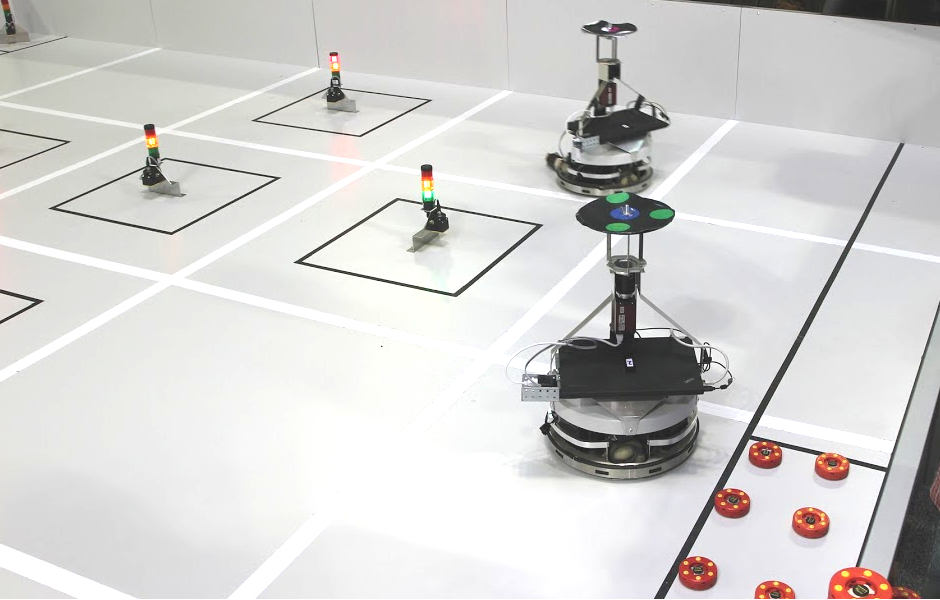
\includegraphics[scale=0.3]{pics/llsf}
\label{Figure 1}
\caption{A half of the LLSF field. Two Robotinos of the Carologistics team at the RoboCup German Open 2013}
\end{figure}
Figure 1 shows a part of the 5.6m x 5.6m hall with two Carologistic robots, three machines and some material-pucks. The main task of LLSF is to produce and deliver ordered products as efficient as possible by feeding machines with resources and semi-finished products. The participants can use up to three Robotino robots by Festo~\cite{{Robotino}}. They hold omni-directional wheels, a gripper to move pucks, and other sensors added by the participants. The orange pucks represent resources and products. They are equipped with an RFID-chip\footnote{Radio-frequency identification allows the wireless identification of objects with small chips.} which is needed to store the different product states of the pucks. The light-signals on top of the RFID-readers represent the machines. They convert resources or semi-finished products into products and trash. There are different types of machines. They can produce different product-types, produce intermediate products, recycle trash or are used for the delivery of products. The light-signals on top of the machines indicate the machine-status. Beside these visual elements, there is also a referee box (refbox), which controls the machines and communicates with the robots during the game. The refbox gives orders which products are to be produced, informs the robots about the game state and rewards points for achieved goals.
\section{Robotino}
\section{Robot Software Frameworks}
\subsection{ROS}
\subsection{Fawkes}
\section{Protocol Buffers}
\section{Gazebo}
\section{MongoDB}
